% Chapter 1

\chapter{Introducción general} % Main chapter title

\label{Chapter1} % For referencing the chapter elsewhere, use \ref{Chapter1} 
\label{IntroGeneral}

En este capítulo se explica en qué consiste la red de domótica empleada, el estado del arte actual, las motivaciones y objetivos propuestos durante la planificación del trabajo.

%----------------------------------------------------------------------------------------

% Define some commands to keep the formatting separated from the content 
\newcommand{\keyword}[1]{\textbf{#1}}
\newcommand{\tabhead}[1]{\textbf{#1}}
\newcommand{\code}[1]{\texttt{#1}}
\newcommand{\file}[1]{\texttt{\bfseries#1}}
\newcommand{\option}[1]{\texttt{\itshape#1}}
\newcommand{\grados}{$^{\circ}$}

%----------------------------------------------------------------------------------------

%\section{Introducción}

%----------------------------------------------------------------------------------------
\section{Domótica en motorhomes}
\label{sec:1_1}
Este trabajo fue desarrollado para la empresa Enertik Argentina \citep{web_enertik}. 
Esta empresa se dedica principalmente a la comercialización de equipos asociados al 
campo de las energías renovables. A su vez, dispone de un área de investigación y 
desarrollo que se especializa en la fabricación y comercialización de equipos 
destinados a la domótica de motorhomes.

Cuando se habla de domotizar un espacio, se hace referencia a la incorporación de 
sistemas electrónicos que permiten automatizar, monitorear y controlar distintos 
parámetros asociados a una unidad habitacional. Estos sistemas buscan mejorar el 
confort del usuario, optimizar el uso de la energía y simplificar la operación de 
los diferentes dispositivos presentes en el entorno.

En el caso particular de los motorhomes, la domótica se aplica al control de 
diferentes subsistemas del vehículo, tales como la iluminación, los sistemas de 
audio, el monitoreo del estado de las baterías, el accionamiento de los motores 
que operan las partes móviles del vehículo y la supervisión de distintos 
parámetros del sistema energético. La integración de estos elementos permite 
centralizar la información y el control de los dispositivos, y así facilitar su 
operación por parte del usuario.

En este contexto, Enertik desarrolla una red de domótica propia destinada 
a la integración y control de los diferentes dispositivos presentes en un 
motorhome. Esta red permite interconectar diversos equipos electrónicos y 
posibilita su supervisión y control mediante una pantalla que permite 
visualizar y operar los distintos dispositivos conectados a la red de domótica.

\section{Motivaciones del trabajo}
\label{sec:1_2}
Fueron varias las motivaciones que impulsaron el desarrollo de este trabajo. 
En primer lugar, dentro de los distintos dispositivos que forman parte de la 
red de domótica del motorhome, existe un subsistema encargado de monitorear 
y gestionar la parte energética del vehículo.

Este sistema se compone principalmente de un conjunto de equipos conformado 
por una batería, un inversor y un cargador.

La batería constituye el dispositivo de almacenamiento de energía del vehículo. 
A partir de ella se alimentan los diferentes equipos eléctricos presentes en 
la unidad.

Por su parte, el inversor es el encargado de transformar la tensión continua 
proveniente de la batería en tensión alterna. Esto permite alimentar dispositivos 
eléctricos que normalmente funcionan conectados a redes eléctricas domiciliarias.

Finalmente, el cargador tiene la función de convertir la tensión alterna 
proveniente de la red eléctrica en una forma adecuada para recargar las 
baterías y almacenar energía en ellas.

En la actualidad se puede observar una tendencia, en donde los fabricantes de motorhomes se encuentran
migrando este conjunto de bateria, cargador e inversor a equipos provistos por la marca Victron Energy \citep{web_victron}.

Esta tendencia fue la principal impulsora en el desarrollo de este trabajo, ya que fue necesario diseñar un
dispositivo que permita acoplar los equipos provistos por la marca Victron a la red de domótica implementada por Enertik.

A su vez, se buscó desarrollar una aplicación que permita darle al usuario una opción adicional (ademas de la pantalla principal) que permita controlar todos los equipos dentro del vehículo, tanto los equipos de la red
de Enertik como así también a los equipos de la red Victron.

De esta manera se buscó solucionar dos problemáticas presentes: por un lado,
la migración hacia nuevas tecnologías energéticas por parte de los fabricantes
de motorhomes y, por otro, la necesidad de brindar a los usuarios nuevas
herramientas para la supervisión y el control del vehículo.

\section{Estado del arte}
\label{sec:1_3}
En la actualidad, Enertik dispone de una estructura bastante bien definida a la hora de domotizar un motorhome. Entre los distintos dispositivos que componen esta red, se destaca uno en particular denominado PRC10 \citep{BOOK:manual_prc10}.

La figura \ref{fig:esquema_domotica} muestra un esquema básico de cómo se compone la red de domótica en la actualidad.

Como se puede apreciar, la arquitectura se basa en un esquema centralizado, donde el
módulo PRC10 actúa como unidad de control principal del sistema. Los
diferentes dispositivos presentes en el vehículo se comunican con este
módulo, que se encarga de procesar la información recibida y ejecutar
las acciones correspondientes sobre los distintos subsistemas.

También se puede observar la presencia de una pantalla táctil que
actúa como interfaz de usuario entre el sistema de domótica y los
ocupantes del vehículo. A través de esta interfaz es posible visualizar
diferentes parámetros obtenidos a partir de los sensores distribuidos en
la unidad, tales como valores asociados al sistema energético, estados
de funcionamiento de los dispositivos conectados y otras variables de
interés para el usuario.

\begin{figure}[h]
	\centering
	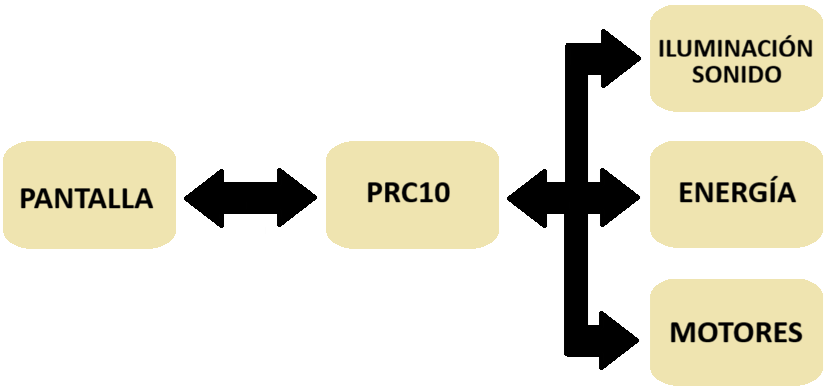
\includegraphics[scale=0.6]{./Figures/esquema_domotica.png}
	\caption{Arquitectura centralizada de la red de domótica con el módulo PRC10 como unidad de control.}
	\label{fig:esquema_domotica}
\end{figure}

\newpage
Además de permitir la supervisión del estado general del sistema, la
pantalla brinda la posibilidad de interactuar con los distintos
periféricos presentes en el motorhome. De esta manera, el usuario puede
realizar acciones de control sobre diversos dispositivos, como la
iluminación, los mecanismos motorizados y otros subsistemas integrados
dentro de la red de domótica.

Entre los distintos dispositivos que componen la red de domótica de Enertik, se destacan los siguientes:

\begin{itemize}
    \item PRC10: módulo central de procesamiento, responsable de la
recepción de información proveniente de los demás dispositivos y de la
toma de decisiones sobre el funcionamiento del sistema. Además, permite
el comando de distintos periféricos, tales como la iluminación interna
del vehículo, la apertura y cierre de esclusas de agua, la activación de
la bomba de agua y el accionamiento de los motores asociados a las
partes móviles del vehículo, como la mesa, la cama levadiza y el toldo.
    \item Pantalla HMI (\textit{Human Machine Interface}): interfaz de usuario de tipo táctil que ejecuta el software principal del sistema. Permite la visualización del estado de las variables y la operación de los distintos dispositivos conectados a la red.
    \item Módulo transceiver: dispositivo que permite la adaptación de la pantalla HMI a la red de comunicación del motorhome.
    \item Módulo sensor de gases: dispositivo encargado de la medición de la composición de gases en el ambiente. Genera alertas ante la detección de condiciones perjudiciales para la salud.
    \item Módulo RGB: módulo de potencia destinado al control de la iluminación RGB distribuida en el vehículo.
    \item Módulo de control de patas: dispositivo responsable del accionamiento del sistema de estabilización del vehículo mediante el control de las patas de apoyo.
    \item Módulo de control de escalón: dispositivo responsable de la operación del mecanismo del escalón de acceso al vehículo.
    \item Módulo de relés para luces vehiculares: dispositivo encargado de la adaptación de niveles de tensión para el control de las luces del vehículo, tales como luces delanteras, traseras y señalización asociada al freno de mano.
    \item Módulo medidor de tanques de agua: módulo encargado de medir y reportar el nivel de llenado de los tanques de agua limpia, gris y negra.

\end{itemize}


\section{Objetivos y alcances}
\label{sec:1_4}
El objetivo del presente trabajo es el desarrollo de un dispositivo que
permita satisfacer dos necesidades principales: por un lado, la
incorporación de nuevas tecnologías a la red de domótica desarrollada
por Enertik y, por otro, brindar a los usuarios una opción adicional
para controlar dicha red mediante una aplicación ejecutable en
dispositivos móviles, tales como teléfonos celulares y tablets.

El microcontrolador elegido para el desarrollo del dispositivo fue el
ESP32 \citep{web_espressif}. Cabe destacar que este equipo no existía al momento de la
planificación inicial del trabajo, por lo que su diseño fue realizado
con la intención de que pueda convertirse posteriormente en un producto
comercial para la empresa.

La figura \ref{fig:esquema_equipo} muestra el esquema de la arquitectura
de comunicación implementada, en la que se destaca la integración del dispositivo
basado en ESP32 como intermediario entre el módulo PRC10, el Cerbo GX y
la aplicación móvil.

Dentro del ecosistema Victron Energy existe un dispositivo denominado
Cerbo GX \citep{web_cerbo_gx}. Este dispositivo actúa como módulo de control principal de la red de
equipos Victron. En este contexto, el dispositivo desarrollado en este
trabajo cumple la función de intermediario entre el módulo Cerbo GX y el
módulo PRC10 perteneciente a la red de domótica de Enertik.

De esta manera, el módulo PRC10 puede acceder a la información generada
por los equipos Victron y, a su vez, controlar ciertas variables que el
sistema pone a disposición a través del módulo Cerbo GX.

Para lograr esta integración fue necesario que el dispositivo de
comunicación sea capaz de manejar diferentes protocolos de comunicación.

En primer lugar, se incorporó el protocolo CAN (\textit{Controller Area Network}) \citep{web_intro_can}, ya que este es el protocolo utilizado en la red de domótica de Enertik. Por otra parte,
Victron pone a disposición documentación técnica en su sitio web
\citep{web_victron_modbus}, donde se describe la forma de controlar el
módulo Cerbo GX mediante el protocolo Modbus TCP \citep{web_intro_modbus}.

Adicionalmente, el dispositivo debía contar con un terminal de cuatro
hilos (+12 V, GND, CAN H y CAN L) con el objetivo de permitir su
conexión directa al mismo cableado utilizado por la red de domótica.
De esta manera, se garantiza tanto su alimentación como el intercambio
de datos.

\begin{figure}[t]
	\centering
	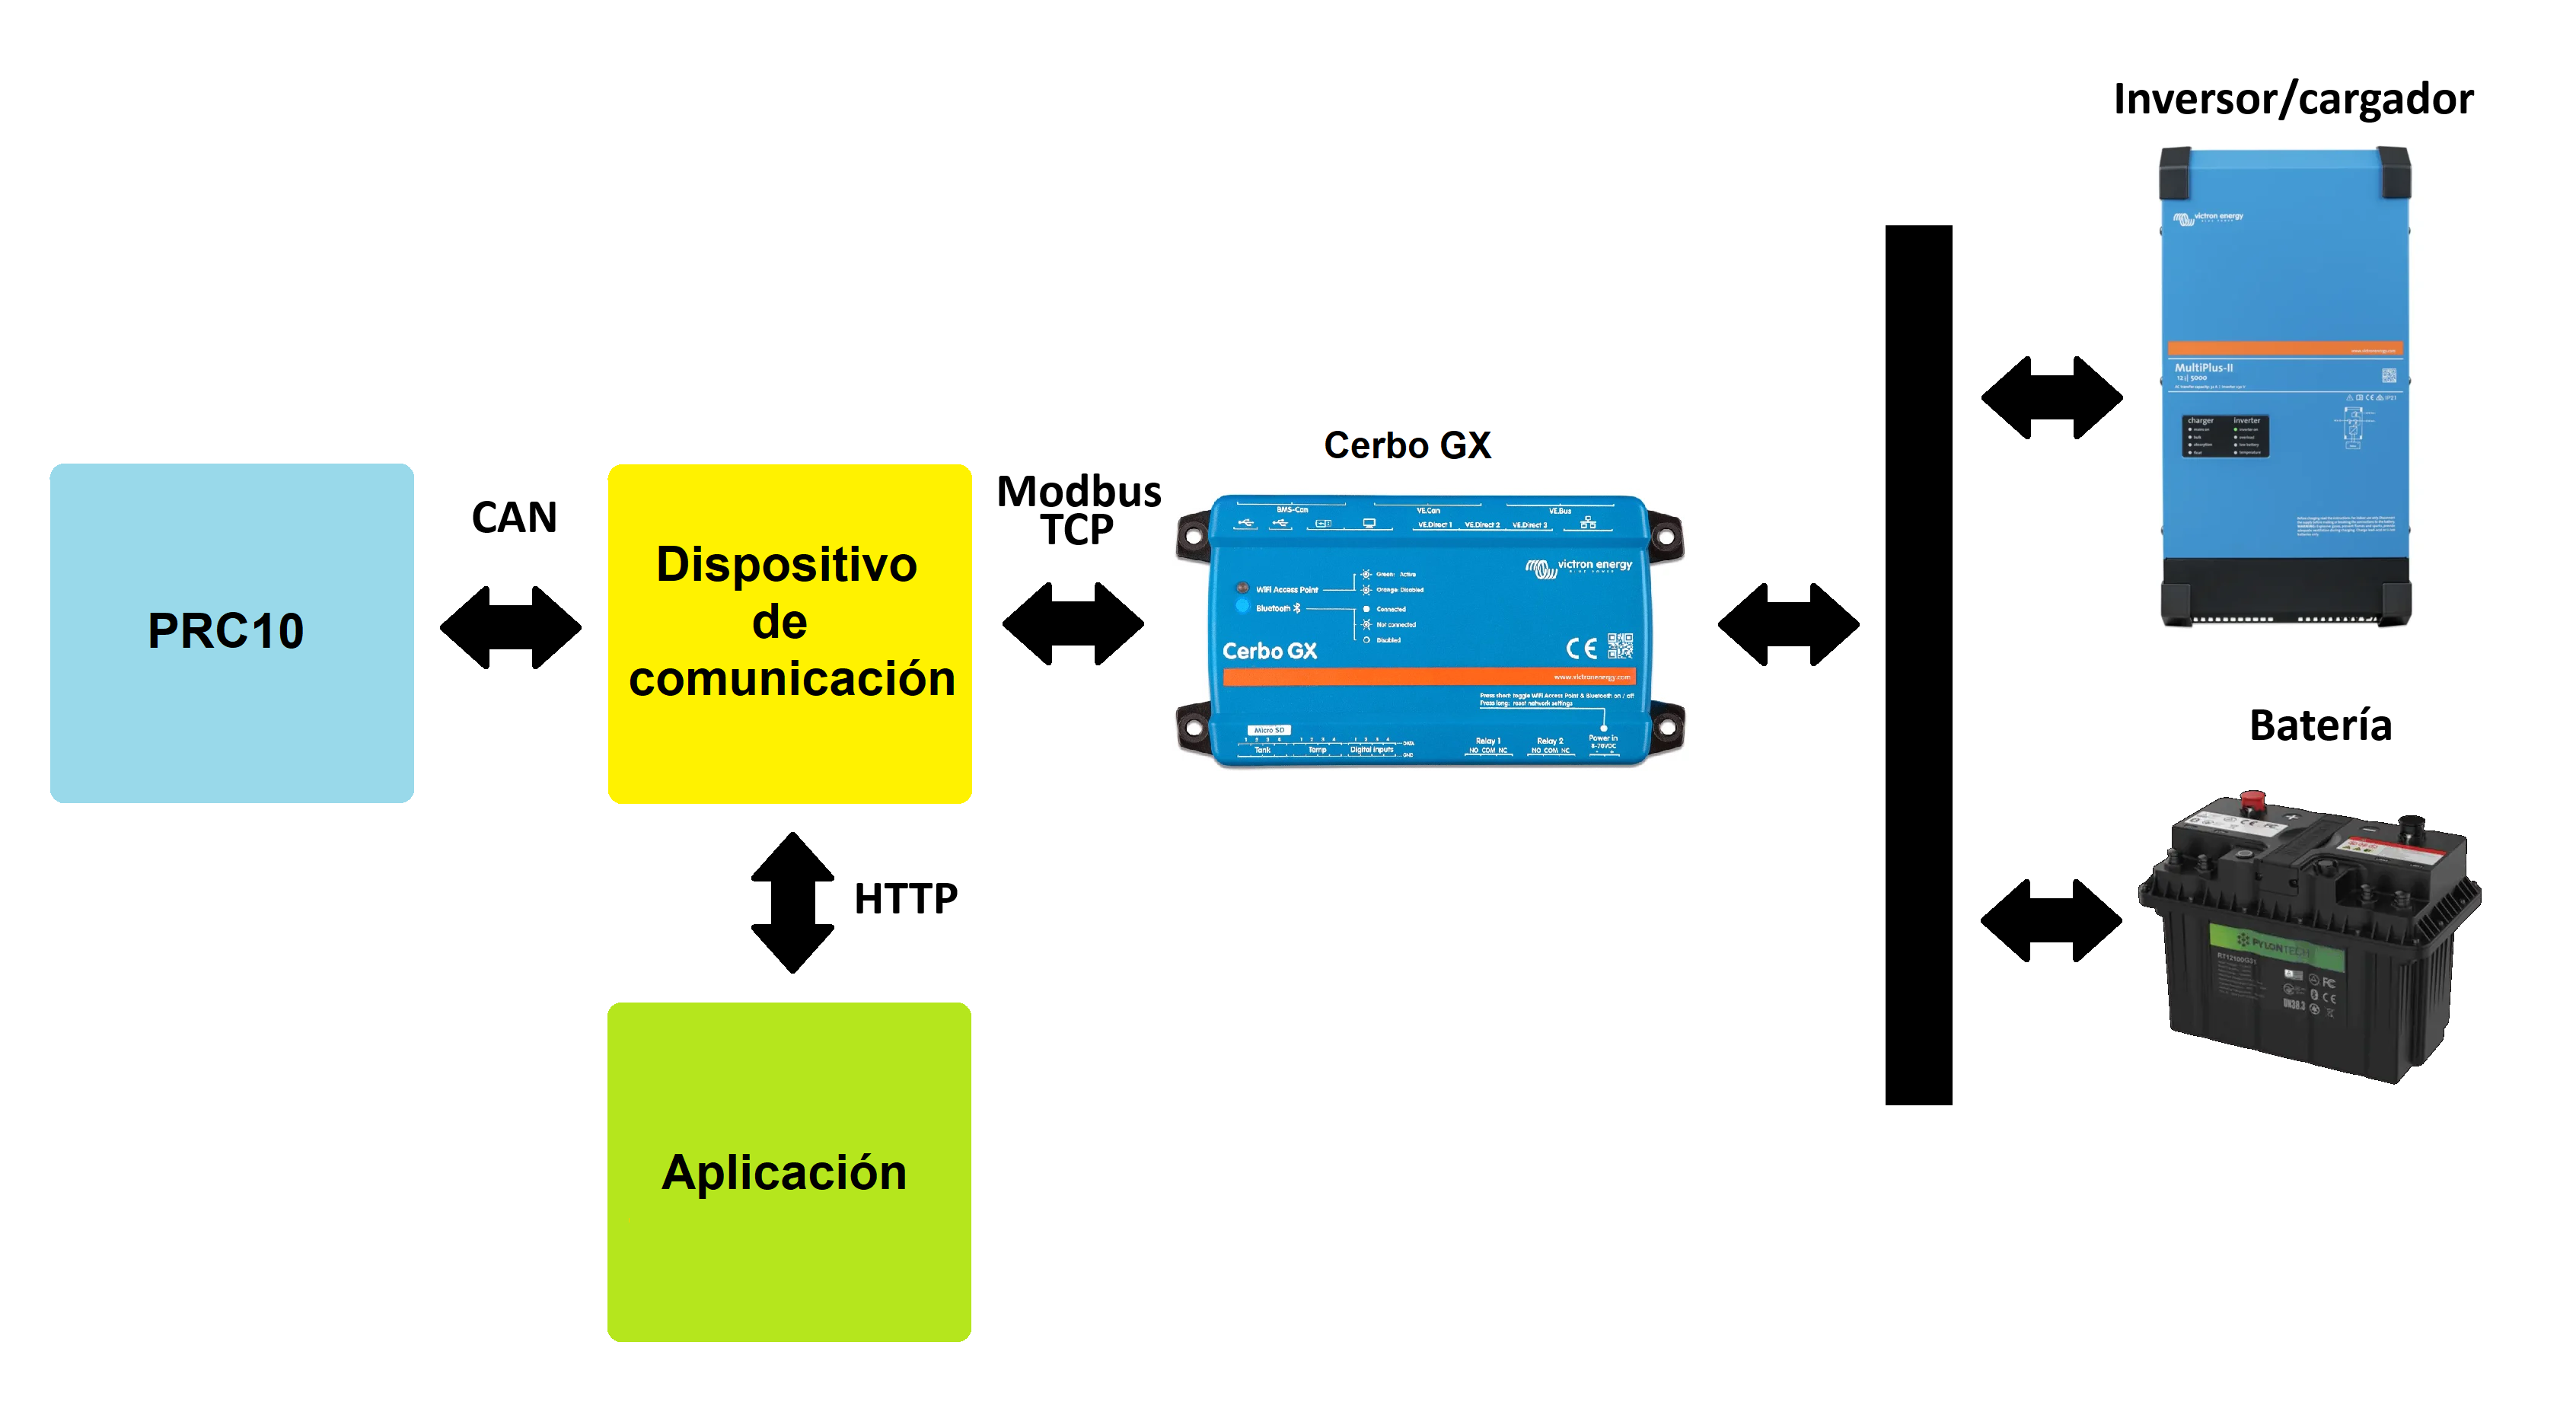
\includegraphics[scale=0.16]{./Figures/esquema.png}
	\caption{Arquitectura de comunicación del sistema con el ESP32 como intermediario entre PRC10, Cerbo GX y la aplicación móvil.}
	\label{fig:esquema_equipo}
\end{figure}
\newpage
En cuanto a la aplicación móvil, se buscó que pueda ejecutarse en
dispositivos portátiles y que sea capaz de comunicarse con el módulo
PRC10 para obtener y mostrar en pantalla las lecturas de las distintas variables del vehículo,
así como también enviar comandos de control hacia los dispositivos
conectados a la red.
